% Decision tree of the Task 3 experiments: what was kept, what was dropped, and the
% result that decided each one. Section numbers refer to TODO.md.
% Compile from inside reports/:  ~/anaconda3/envs/tex/bin/tectonic decision_tree.tex
\documentclass[10pt,a4paper]{article}

\usepackage[margin=10mm]{geometry}
\usepackage{tikz}
\usepackage{xcolor}
\usepackage[colorlinks=true,linkcolor=black,urlcolor=black]{hyperref}
\usetikzlibrary{positioning,arrows.meta,calc}

\definecolor{keep}{HTML}{2C7A5A}
\definecolor{keepfill}{HTML}{E8F3ED}
\definecolor{drop}{HTML}{9AA5B1}
\definecolor{dropfill}{HTML}{F5F7FA}
\definecolor{live}{HTML}{B45309}
\definecolor{livefill}{HTML}{FDF3E3}
\definecolor{ink}{HTML}{102A43}
\definecolor{muted}{HTML}{627D98}

\pagestyle{empty}
\setlength{\parindent}{0pt}

\tikzset{
  kept/.style = {draw=keep, fill=keepfill, line width=0.7pt, rounded corners=1.2pt,
                 text width=44mm, inner sep=1.6mm, align=left, font=\footnotesize},
  gone/.style = {draw=drop, fill=dropfill, line width=0.4pt, dashed, rounded corners=1.2pt,
                 text width=58mm, inner sep=1.3mm, align=left, font=\scriptsize, text=muted},
  back/.style = {draw=keep, fill=dropfill, line width=0.5pt, dashed, rounded corners=1.2pt,
                 text width=58mm, inner sep=1.3mm, align=left, font=\scriptsize, text=keep},
  now/.style  = {draw=live, fill=livefill, line width=0.7pt, rounded corners=1.2pt,
                 text width=44mm, inner sep=1.5mm, align=left, font=\footnotesize},
  spine/.style = {->, draw=keep, line width=1.1pt, >={Stealth[length=2mm]}},
  stub/.style  = {->, draw=drop, line width=0.4pt, dashed, >={Stealth[length=1.4mm]}},
  ret/.style   = {->, draw=keep, line width=0.5pt, dashed, >={Stealth[length=1.4mm]}},
  sec/.style   = {font=\footnotesize\bfseries, text=ink},
}

% #1 node name, #2 y, #3 section, #4 what it was, #5 result
\newcommand{\kept}[5]{\node[kept] (#1) at (0,#2)
  {{\bfseries #3}~~#4\\[0.4mm]{\bfseries\color{keep}#5}};}
\newcommand{\gone}[5]{\node[gone] (#1) at (7.6,#2)
  {\hyphenpenalty=10000\exhyphenpenalty=10000\relax
   {\bfseries #3}~~#4 \hfill \textbf{#5}};}
\newcommand{\back}[5]{\node[back] (#1) at (7.6,#2)
  {\hyphenpenalty=10000\exhyphenpenalty=10000\relax
   {\bfseries #3}~~#4 \hfill \textbf{#5}};}
\newcommand{\note}[2]{\node[font=\scriptsize\itshape, text=muted, text width=34mm, align=right]
  at (-4.4,#1) {#2};}

\begin{document}

{\Large\bfseries What we tried, what we kept}\\[1mm]
{\small Task 3, team \texttt{inzva\_mri}, to 2026-09-14. \textcolor{keep}{Green spine} = changes that
shipped, \textcolor{drop}{grey stubs} = tried and dropped, \textcolor{keep}{green dashed} = dropped on a
local number and later shipped, \textcolor{live}{orange} = built, not yet scored.
Section numbers are \texttt{TODO.md}. Scores are challenge SSIM; deltas are local, and every local
delta dated before 2026-09-11 was measured on the wrong plane (page 2).}\\[3mm]

\begin{center}
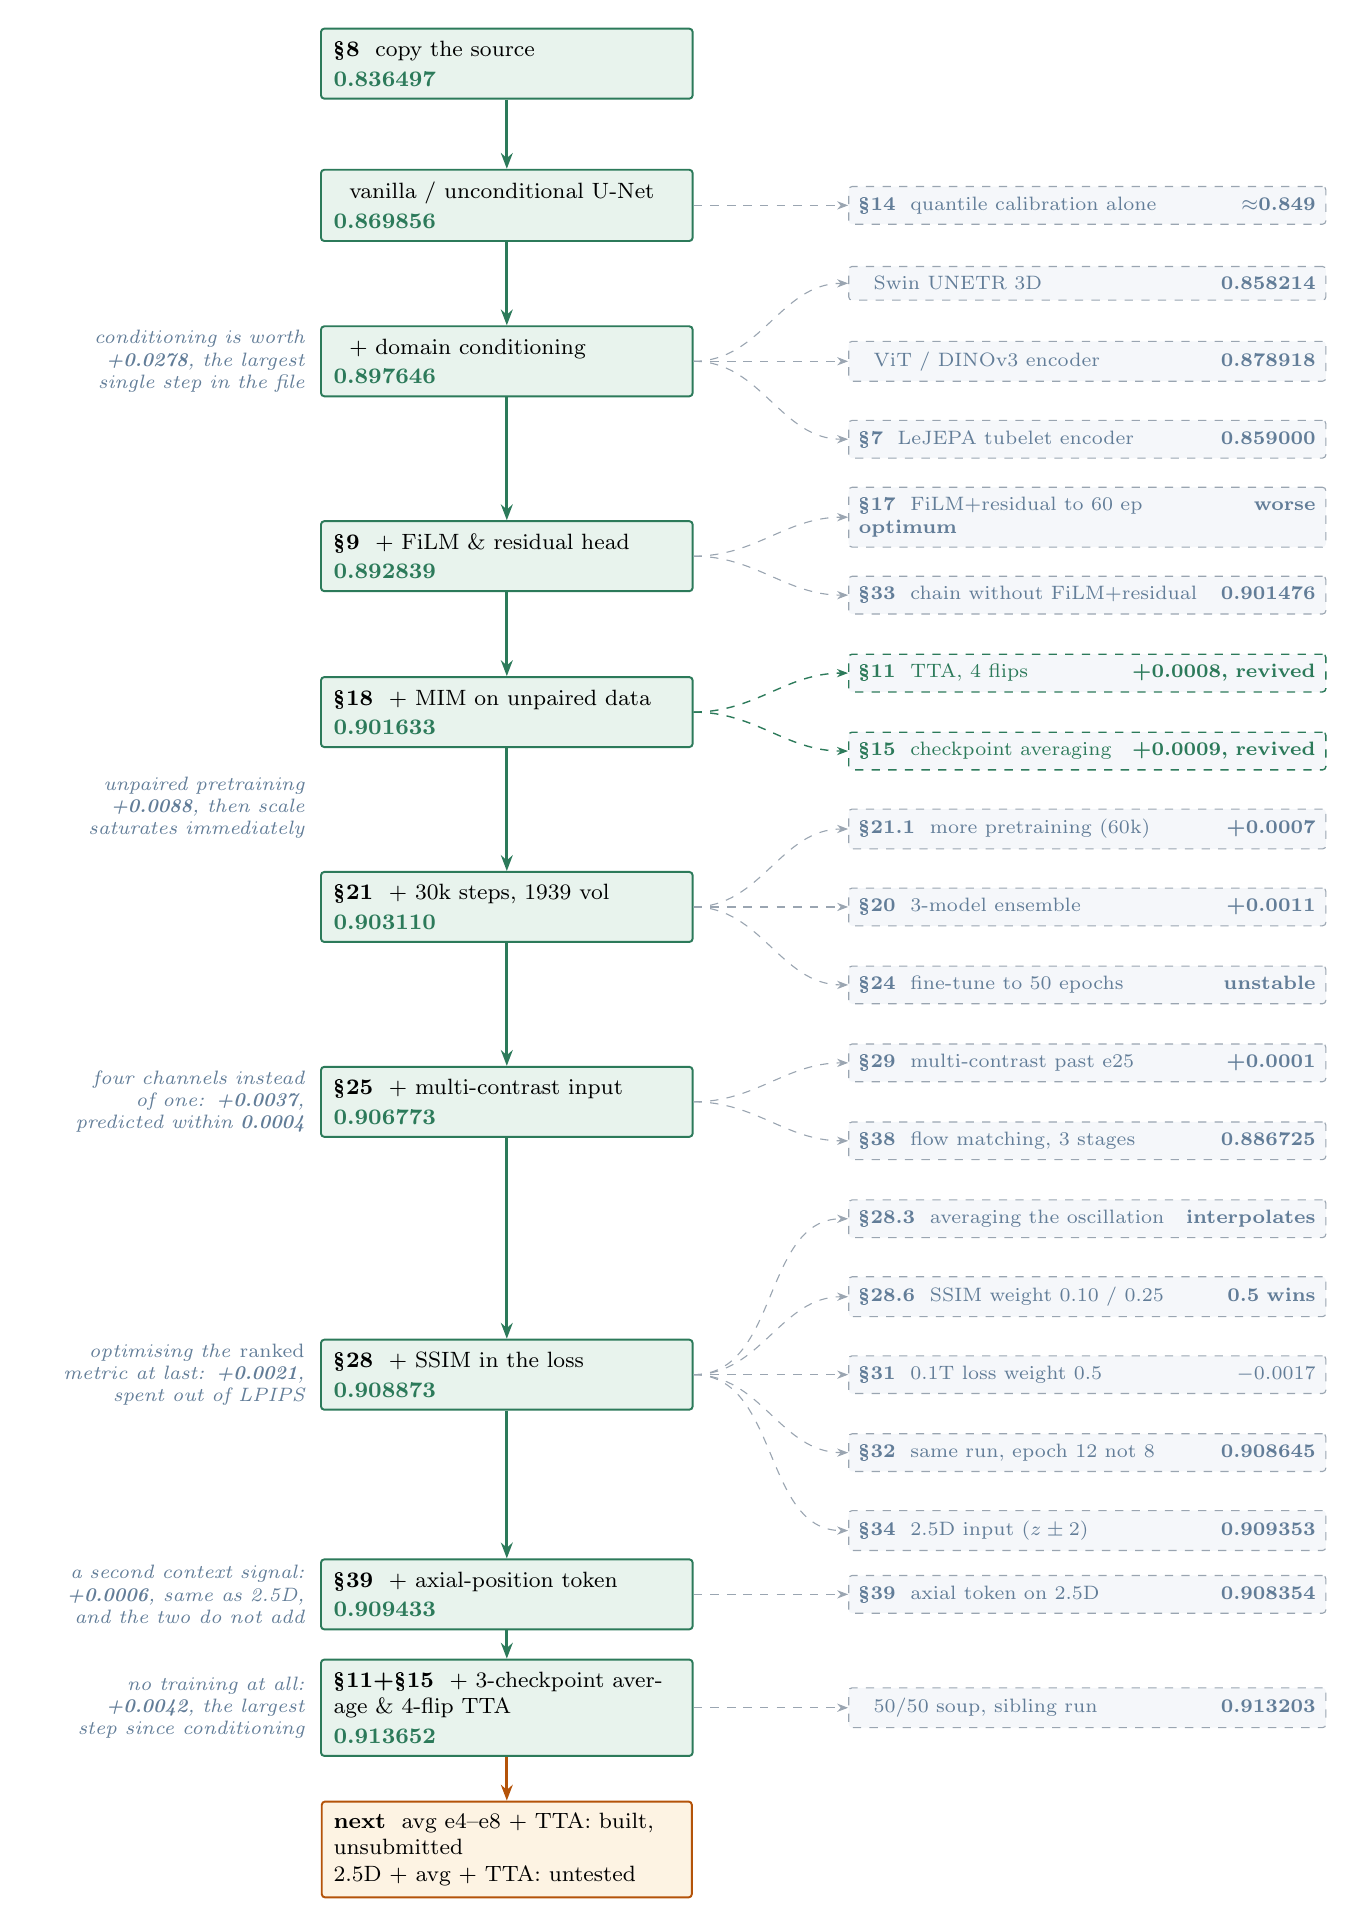
\begin{tikzpicture}[x=0.97cm,y=0.90cm]

% ------------------------------------------------------------------ the spine
\kept{n1}{0}      {\S8}   {copy the source}              {0.836497}
\kept{n2}{-2.0}   {}      {vanilla / unconditional U-Net} {0.869856}
\kept{n3}{-4.2}   {}      {+ domain conditioning}        {0.897646}
\kept{n4}{-6.95}  {\S9}   {+ FiLM \& residual head}      {0.892839}
\kept{n5}{-9.15}  {\S18}  {+ MIM on unpaired data}       {0.901633}
\kept{n6}{-11.9}  {\S21}  {+ 30k steps, 1939 vol}        {0.903110}
\kept{n7}{-14.65} {\S25}  {+ multi-contrast input}       {0.906773}
\kept{n8}{-18.5}  {\S28}  {+ SSIM in the loss}           {0.908873}
\kept{n9}{-21.6}  {\S39}  {+ axial-position token}       {0.909433}
\kept{n10}{-23.2} {\S11+\S15} {+ 3-checkpoint average \& 4-flip TTA} {0.913652}
\node[now] (n11) at (0,-25.2)
  {{\bfseries next}~~avg e4--e8 + TTA: built, unsubmitted\\
   2.5D + avg + TTA: untested};

\foreach \a/\b in {n1/n2, n2/n3, n3/n4, n4/n5, n5/n6, n6/n7, n7/n8, n8/n9, n9/n10}{\draw[spine] (\a) -- (\b);}
\draw[spine, draw=live] (n10) -- (n11);

% ------------------------------------------------------------------ dropped
\gone{d1}{-2.0}  {\S14} {quantile calibration alone}    {$\approx$0.849}
\gone{d2}{-3.1}  {}     {Swin UNETR 3D}                 {0.858214}
\gone{d3}{-4.2}  {}     {ViT / DINOv3 encoder}          {0.878918}
\gone{d4}{-5.3}  {\S7}  {LeJEPA tubelet encoder}        {0.859000}
\gone{d5}{-6.4}  {\S17} {FiLM+residual to 60 ep}        {worse optimum}
\gone{d6}{-7.5}  {\S33} {chain without FiLM+residual}   {0.901476}
\back{d7}{-8.6}  {\S11} {TTA, 4 flips}                  {+0.0008, revived}
\back{d8}{-9.7}  {\S15} {checkpoint averaging}          {+0.0009, revived}
\gone{d9}{-10.8} {\S21.1}{more pretraining (60k)}       {+0.0007}
\gone{d10}{-11.9}{\S20} {3-model ensemble}              {+0.0011}
\gone{d11}{-13.0}{\S24} {fine-tune to 50 epochs}        {unstable}
\gone{d12}{-14.1}{\S29} {multi-contrast past e25}       {+0.0001}
\gone{d13}{-15.2}{\S38} {flow matching, 3 stages}       {0.886725}
\gone{d14}{-16.3}{\S28.3}{averaging the oscillation}    {interpolates}
\gone{d15}{-17.4}{\S28.6}{SSIM weight 0.10 / 0.25}      {0.5 wins}
\gone{d16}{-18.5}{\S31} {0.1T loss weight 0.5}          {$-0.0017$}
\gone{d17}{-19.6}{\S32} {same run, epoch 12 not 8}      {0.908645}
\gone{d18}{-20.7}{\S34} {2.5D input ($z\pm2$)}          {0.909353}
\gone{d19}{-21.6}{\S39} {axial token on 2.5D}           {0.908354}
\gone{d20}{-23.2}{}     {50/50 soup, sibling run}       {0.913203}

\draw[stub] (n2.east) to[out=0,in=180] (d1.west);
\foreach \d in {d2,d3,d4}{\draw[stub] (n3.east) to[out=0,in=180] (\d.west);}
\foreach \d in {d5,d6}{\draw[stub] (n4.east) to[out=0,in=180] (\d.west);}
\foreach \d in {d7,d8}{\draw[ret] (n5.east) to[out=0,in=180] (\d.west);}
\foreach \d in {d9,d10,d11}{\draw[stub] (n6.east) to[out=0,in=180] (\d.west);}
\foreach \d in {d12,d13}{\draw[stub] (n7.east) to[out=0,in=180] (\d.west);}
\foreach \d in {d14,d15,d16,d17,d18}{\draw[stub] (n8.east) to[out=0,in=180] (\d.west);}
\draw[stub] (n9.east) to[out=0,in=180] (d19.west);
\draw[stub] (n10.east) to[out=0,in=180] (d20.west);

% ------------------------------------------------------------------ annotations
\note{-4.2}  {conditioning is worth\\ \textbf{+0.0278}, the largest\\ single step in the file}
\note{-10.5} {unpaired pretraining\\ \textbf{+0.0088}, then scale\\ saturates immediately}
\note{-14.65}{four channels instead\\ of one: \textbf{+0.0037},\\ predicted within \textbf{0.0004}}
\note{-18.5} {optimising the \emph{ranked}\\ metric at last: \textbf{+0.0021},\\ spent out of LPIPS}
\note{-21.6} {a second context signal:\\ \textbf{+0.0006}, same as 2.5D,\\ and the two do not add}
\note{-23.2} {no training at all:\\ \textbf{+0.0042}, the largest\\ step since conditioning}

\end{tikzpicture}
\end{center}

\newpage
{\footnotesize\setlength{\parskip}{1.6mm}
\textbf{How to read the stubs.} Every grey branch was measured, not guessed, and most were
killed by a number rather than by taste. Three of them (\S11, \S15, \S20) were real but read
too small: $+0.0008$ to $+0.0011$ local, against a seed noise floor of $\pm0.001$ (\S16) and a
between-subject spread of $0.011$ (\S14.1). The reasoning was right about the ruler and wrong
about the effect; see the next paragraph.

\textbf{Two stubs came back, and the ruler was the reason.} Until 2026-09-11
\texttt{eval\_holdout.py} walked axis 0 of the cached volume and fed every 2D model
\emph{sagittal} $436\times364$ planes, while training and the submission path cut axial
$364\times436$ ones; the transpose existed only as an opt-in flag that the two tubelet configs
set. Nothing errored: both axes are 364 long and the network is fully convolutional. On that
ruler TTA and checkpoint averaging read $+0.0017$ combined and were declined twice; submitted
together on 2026-09-11 they scored $+0.0042$, the largest single step since conditioning. The
same ruler picked \S32's epoch 12 by every check it had and lost, and ranked the SSIM-loss
family backwards from the leaderboard. Fixed; the harness now reproduces the submission path
to $1.8\cdot10^{-4}$. Every local delta on page 1 is a sagittal-plane number: read it as a
sign at best, not a magnitude. The challenge scores are unaffected.

\textbf{The one branch that was on the spine but should have been a stub is settled.} \S9's
FiLM+residual head scored \emph{below} the plain conditional U-Net it replaced ($-0.0048$) and
\S17's 60-epoch run confirmed a worse optimum, so the pretraining line was suspected of
carrying a $\approx0.005$ cost. \S33 re-ran the whole chain with the two flags off and nothing
else changed: \textbf{0.901476}, against 0.901633 (12k pretrain) and 0.903110 (30k) with them
on. On unseen subjects FiLM+residual is worth $+0.0016$; the $-0.0048$ was training-subject
fit, measured on the wrong plane besides. Closed.

\textbf{What the shape of the tree says.} Every stub on the right is an \emph{architecture},
a \emph{schedule}, or a second helping of something already on the spine. Every step on the
spine after the U-Net exists is a change in what the model gets to \emph{see} (which domains
it maps between, 1{,}939 volumes with no paired target, the other two contrasts, where in the
head the slice sits) until the last one, which changes nothing the model sees and only how
many of its own estimates are averaged. With three paired subjects, information is the binding
constraint; and once the information is in, the remaining gain was variance. \S28 is the one
exception and the first step to optimise the \emph{ranked} metric directly rather than a proxy
for it.

\textbf{Context signals saturate at one.} The neighbouring-slice input (\S34, $+0.0005$ over
its parent) and the axial-position token (\S39, $+0.0006$) are within $0.0001$ of each other
and, combined on the 2.5D branch, score $-0.0010$ under it. The spine took the token because
that is the run that was averaged; the 2.5D branch with the same averaging is the untested
orange item.

\textbf{The flow-matching branch (\S38) is closed with a leaderboard number.} The rank-1
team's recipe (degradation-bridge pretraining on 232k retrospective slices, conditional
flow matching, GAN refinement, 5 Heun steps, 4-flip TTA) reproduced end to end scored
\textbf{0.886725}, below every conditioned U-Net in the file and worse on all three metrics.
The paper's own complete-pipeline number is 0.909; the regression U-Net was already there
before the branch was started.

\smallskip
\textbf{\S28 nearly became a stub by accident.} Scored first at epoch 10, on a checkpoint grid
inherited from a run whose peak was at epoch 20, it read 0.9527 against a matched 0.95706 and
looked dead. Epoch 5 scored 0.9598. The trajectory swings 0.951--0.961 between adjacent epochs,
so one checkpoint of an unswept schedule was never evidence about the lever, only about that
checkpoint. (Sagittal-plane numbers; the swing has not been re-measured on the fixed harness.)}

\end{document}
